\documentclass{TDP005mall}



\newcommand{\version}{Version 0.1}
\author{Niklas Åsberg, \url{nikas214@student.liu.se}}
\title{Designspecifikation}
\date{2023-11-21}
\rhead{Niklas Åsberg}
\graphicspath{{./}}

\begin{document}
\projectpage
\section{Revisionshistorik}
\begin{table}[!h]
\begin{tabularx}{\linewidth}{|l|X|l|}
\hline
Ver. & Revisionsbeskrivning & Datum \\\hline
0.1 & Utkast & 2023-11-21 \\\hline
\end{tabularx}
\end{table}

\tableofcontents
\newpage

\section{Introduction}
I det här dokumentet så beskrivs designen av mitt spel. Jag kommer att gå igenom två av mina klasser i detalj och sen visa UML-diagrammet över alla mina klasser. \\
Avslutningsvis diskuterar jag mina designval.

\section{Detaljbeskrivning}
Två av mina klasser kan vara extra intressanta att analysera: Playerklassen och Squareklassen.

\subsection{Playerklassen}
Playerklassen ska representera spelaren. Klassen implementerar Characterklassen som i sin tur ärver från GameObjectklassen. \\
Playerklassen interagerar direkt med en annan klass, Squareklassen. 
\subsubsection{Attribut}
Dessa attribut är specificerade i Characterklassen som är en interface som i sin tur ärver av GameObjectklassen.
\begin{itemize}
  \item int: health - antalet liv spelaren har.
  \item float: speed - hur snabbt spelaren kan röra sig.
  \item int: damage - hur mycket skada spelaren gör när den attackerar.
  \item sf::vector2f: prevLocation - den senaste rutan spelaren var på.
  \item sf::vector2f: location - rutan som spelaren är på just nu.
  \item string: sprite - filvägen till spelarens bild.
  \item bool: collidable - bool som visar om det går att kollidera med spelaren
\end{itemize}
\subsubsection{Metoder}
Metoden attack() är den enda metoden som är unik för Playerklassen, de andra metoderna är specificerade i interfacet.
\begin{itemize}
  \item onCollision() - vad som händer om en spelare kolliderar med någonting annat.
  \item move() - metod för att flytta spelaren.
  \item attack() - metod för att attackera.
\end{itemize}

\newpage

\subsection{Squareklassen}
Squareklassen representerar en ruta på spelplanen. En ruta kan innehålla ett eller inga objekt som implementerar GameObjectklassen. \\
Squareklassen interagerar direkt med objekt som implementerar GameObjectklassen och Mapklassen. Mapklassen innehåller flera instanser av Squareklassen. \\
\subsubsection{Attribut}
\begin{itemize}
  \item GameObject: contains - en referens till vilket objekt som står på den här rutan.
  \item sf::vector2f: location - positionen för den här rutan.
\end{itemize}
\subsubsection{Metoder}
\begin{itemize}
  \item canBeMovedTo() - anropas av ett objekt som vill flytta till den här rutan för att se om rutan redan är upptagen eller inte.
\end{itemize}

\section{UML-diagram}
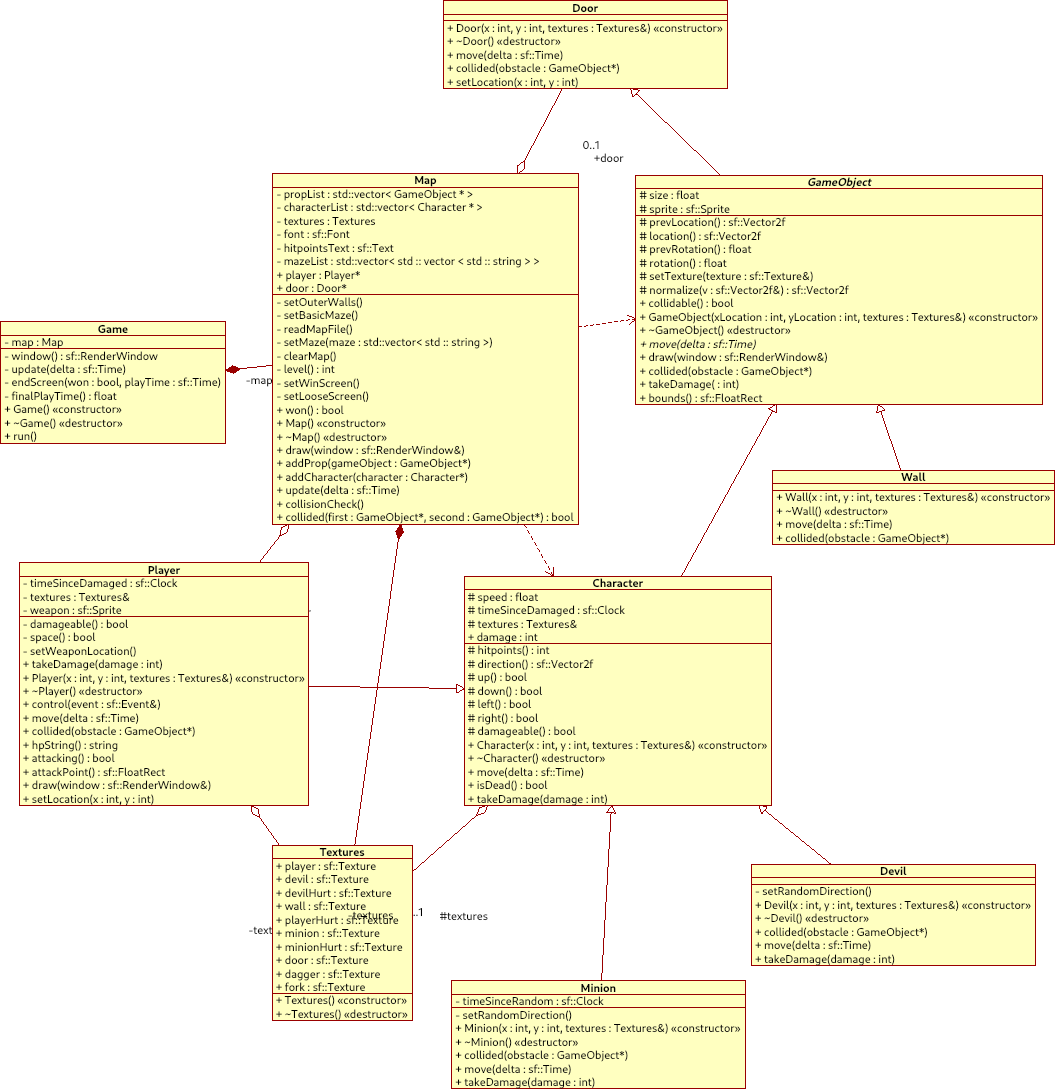
\includegraphics[scale=0.52]{uml-diagram}

\newpage
\section{Diskution}
I mitt spel så utgår allt från en instans av Gameklassen, Gameklassen innehåller en instans av Mapklassen. Gameklassen har även ansvaret att byta instansen \\
av map när en ny bana påbörjas, Gameklassen sköter inladdningen av ban-filen och skapar Map-instansen från den. 
Map-instansen innehåller alla Square-instanser. Squareklassen har sen koll på alla GameObject-instanser.
Jag valde den här typen av design då det blir väldigt lätt att lägga till och ändra hur spelet ska se ut. \\
Om man till exempel vill lägga till andra hinder eller karaktärer så behöver vi inte ändra i de allra flesta klasser.
Kollisionshanteringen sker mellan spelobjekt så om vi skulle vilja ändra vad som händer vid kollision så ändrar vi bara i det spelobjektets klass.
Tanken är att minska coupling och ha hög cohesion.

\section{Externa filformat}
Om vi bortser från png-filerna som bara är där för esteriska skäl så är det enda externa filformatet det för banorna.
Mitt spel använder sig av en enkel fil där specifikationen för banan är skiven i text, ett tecken för varje ruta med olika tecken för varje objekt.

\end{document}
